% $Id$
%

\section{Hojas de estilo CSS}


%% LICENCIA DE REDISTRIBUCION DE LAS TRANSPAS
\frame{
~
\vspace{1cm}

\begin{flushright}
\copyright Javier Eguiluz - Librosweb.es \\
\copyright Gregorio Robles - Universidad Rey Juan Carlos \\
\vspace{1cm}

Algunos derechos reservados. Este artículo se distribuye bajo
la licencia ``Reconocimiento-NoComercial-NoObrasDerivadas 3.0 España'' de Creative Commons,
disponible en \\
{\small \url{http://creativecommons.org/licenses/by-nc-nd/3.0/es/deed.es}}
\vspace{1cm}

Este documento se basa en el libro de librosweb.es \\
disponible en http://www.librosweb.es/css/ \\
Se ha pedido explícitamente autorización al autor original \\
para realizar esta obra derivada con fines educativos.
\end{flushright}
}


%%---------------------------------------------------------------

\begin{frame}
\frametitle{¿Qué es CSS?}

\begin{itemize}
  \item Es un lenguaje de hojas de estilos creado para controlar el aspecto o presentación de los documentos electrónicos definidos con HTML y XHTML
  \item Es la mejor forma de separar los contenidos y su presentación y es imprescindible para crear páginas web complejas
  \begin{itemize}
    \item Obliga a crear documentos HTML/XHTML bien definidos y con significado completo (también llamados "documentos semánticos")
    \item Mejora la accesibilidad del documento
    \item Reduce la complejidad de su mantenimiento
    \item Permite visualizar el mismo documento en infinidad de dispositivos diferentes
  \end{itemize}
\end{itemize}

\end{frame}

%%---------------------------------------------------------------

\begin{frame}[fragile]
\frametitle{Antes del CSS}

{\footnotesize
\begin{verbatim}
<!DOCTYPE html PUBLIC "-//W3C//DTD XHTML 1.0 Transitional//EN"
 "http://www.w3.org/TR/xhtml1/DTD/xhtml1-transitional.dtd">
<html xmlns="http://www.w3.org/1999/xhtml">
<head>
 <meta http-equiv="Content-Type" content="text/html; charset=iso-8859-1"/>
 <title>Ejemplo de estilos sin CSS</title>
</head>
 
<body>
 <h1><font color="red" face="Arial" size="5">
    Titular de la página
 </font></h1>
 <p><font color="gray" face="Verdana" size="2">
   Un párrafo de texto no muy largo.
 </font></p>
</body>
</html>
\end{verbatim}
}

\end{frame}

%%---------------------------------------------------------------

\begin{frame}[fragile]
\frametitle{Con CSS}

{\footnotesize
\begin{verbatim}
<!DOCTYPE html PUBLIC "-//W3C//DTD XHTML 1.0 Transitional//EN"
  "http://www.w3.org/TR/xhtml1/DTD/xhtml1-transitional.dtd">
<html xmlns="http://www.w3.org/1999/xhtml">
<head>
<meta http-equiv="Content-Type" content="text/html; charset=iso-8859-1"/>
<title>Ejemplo de estilos con CSS</title>
<style type="text/css">
  h1 { color: red;  font-family: Arial;   font-size: large;  }
  p  { color: gray; font-family: Verdana; font-size: medium; }
</style>
</head>
 
<body>
  <h1>Titular de la página</h1>
  <p>Un párrafo de texto no muy largo.</p>
</body>
</html>
\end{verbatim}
}

\end{frame}

%%---------------------------------------------------------------

\begin{frame}
\frametitle{Incluir un CSS en un documento (X)HTML}

\begin{enumerate}
  \item Incluir CSS en el mismo documento HTML
  \item Definir CSS en un archivo externo
  \item Incluir CSS en los elementos HTML
\end{enumerate}

\end{frame}

%%---------------------------------------------------------------

\begin{frame}
\frametitle{Glosario Básico (I)}

\begin{center}
\begin{figure}[p]
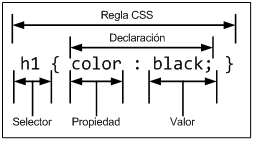
\includegraphics[width=0.6\textwidth]{img/f0101.png}
\end{figure}
\end{center}

\begin{itemize}
  \item Regla: cada uno de los estilos que componen una hoja de estilos CSS. Cada regla está compuesta de una parte de "selectores", un símbolo de ''llave de apertura'' (\{), otra parte denominada ''declaración'' y por último, un símbolo de ''llave de cierre'' (\}).
  \item Selector: indica el elemento o elementos HTML a los que se aplica la regla CSS.
\end{itemize}

\end{frame}

%%---------------------------------------------------------------

\begin{frame}
\frametitle{Glosario Básico (y II)}

\begin{center}
\begin{figure}[p]
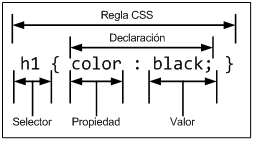
\includegraphics[width=0.42\textwidth]{img/f0101.png}
\end{figure}
\end{center}

\begin{itemize}
  \item Declaración: especifica los estilos que se aplican a los elementos. Está compuesta por una o más propiedades CSS.
  \item Propiedad: característica que se modifica en el elemento seleccionado, como por ejemplo su tamaño de letra, su color de fondo, etc.
  \item Valor: establece el nuevo valor de la característica modificada en el elemento.
\end{itemize}

CSS 2.1 define 115 propiedades y CSS 3 define 239 propiedades.

\end{frame}

%%---------------------------------------------------------------

\begin{frame}
\frametitle{Medios CSS}

\begin{itemize}
  \item Permiten definir diferentes estilos para diferentes medios o dispositivos: pantallas, impresoras, móviles, proyectores, etc.
  \item Define algunas propiedades específicamente para determinados medios: la paginación y los saltos de página para los medios impresos o el volumen y tipo de voz para los medios de audio.
  \item Ejemplos:
  \begin{itemize}
    \item screen: Pantallas de ordenador
    \item print: Impresoras y navegadores en el modo ''Vista Previa para Imprimir''
    \item handheld:	Dispositivos de mano: móviles, PDA, etc.
  \end{itemize}
\end{itemize}

\end{frame}

%%---------------------------------------------------------------

\begin{frame}[fragile]
\frametitle{Formas de indicar el medio}

\begin{enumerate}
  \item Reglas de tipo @media
{\footnotesize
    \begin{verbatim}
@media print {
  body { font-size: 10pt }
}
@media screen {
  body { font-size: 13px }
}
    \end{verbatim}
}
  \item Reglas de tipo @import
{\footnotesize
    \begin{verbatim}
@import url("estilos_basicos.css") screen;
@import url("estilos_impresora.css") print;
    \end{verbatim}
}
  \item Medios definidos con la etiqueta
{\footnotesize
    \begin{verbatim}
<link rel="stylesheet" type="text/css" media="screen" href="basico.css" />
<link rel="stylesheet" type="text/css" media="print, handheld" href="especial.css" />
    \end{verbatim}
}
  \item Medios definidos mezclando varios métodos
{\footnotesize
    \begin{verbatim}
<link rel="stylesheet" type="text/css"  media="screen" href="basico.css" />
@import url("estilos_seccion.css") screen;
@media print {
  /* Estilos específicos para impresora */
}
    \end{verbatim}
}
\end{enumerate}

\end{frame}

%%---------------------------------------------------------------

\begin{frame}[fragile]
\frametitle{Comentarios}

\begin{itemize}
  \item El comienzo de un comentario se indica mediante los caracteres /* y el final del comentario se indica mediante */
    \begin{verbatim}
/* Este es un comentario en CSS */
    \end{verbatim}
  \item Pueden ocupar tantas líneas como sea necesario, pero no se puede incluir un comentario dentro de otro comentario
    \begin{verbatim}
/* Este es un
   comentario CSS de varias
   lineas */
    \end{verbatim}
\end{itemize}

\end{frame}

%%---------------------------------------------------------------

\begin{frame}
\frametitle{Sintaxis}

\begin{itemize}
  \item Sucesión de palabras sin ningún carácter que las separe (paréntesis, comas, barras, etc.) el valor de la propiedad se debe indicar tal y como se muestra y con esas palabras en el mismo orden.
  \item Sucesión de valores separados por una barra simple el valor de la propiedad debe tomar uno y sólo uno de los valores indicados
  \item Sucesión de valores separados por una barra doble el valor de la propiedad puede tomar uno o más valores de los indicados y en cualquier orden.
  \item Cada valor o agrupación de valores se puede indicar el tipo de valor: opcional, obligatorio, múltiple o restringido.
  \item Más: * = cero o más veces; + = una o más veces; ? = opcional; {n1, n2} = entre n1 y n2 veces
\end{itemize}

\end{frame}


%%---------------------------------------------------------------

\section{Selectores}

\begin{frame}
\frametitle{}

\begin{itemize}
  \item A un mismo elemento HTML se le pueden aplicar varias reglas 
  \item Cada regla puede aplicarse a un número ilimitado de elementos
  \item Cuando el selector de dos o más reglas CSS es idéntico, se pueden agrupar las declaraciones de las reglas para hacer las hojas de estilos más eficientes
  \item Cuando se establece el valor de una propiedad CSS en un elemento, sus elementos descendientes heredan de forma automática el valor de esa propiedad
\end{itemize}

CSS 2.1 incluye una docena de tipos diferentes de selectores, que permiten seleccionar de forma muy precisa elementos individuales o conjuntos de elementos dentro de una página web.

\end{frame}

%%---------------------------------------------------------------

\begin{frame}
\frametitle{Selectores básicos}

\begin{enumerate}
  \item Selector universal
  \item Selector de tipo o etiqueta
  \item Selector descendente
  \item Selector de clase
  \item Selector de identidad
\end{enumerate}

\end{frame}

%%---------------------------------------------------------------

\begin{frame}[fragile]
\frametitle{Selector Universal}

\begin{itemize}
  \item No se utiliza habitualmente, ya que es difícil que un mismo estilo se pueda aplicar a todos los elementos de una página.
  \item Se suele combinar con otros selectores y además, forma parte de algunos hacks muy utilizados
\end{itemize}

\begin{verbatim}
* {
  margin: 0;
  padding: 0;
}
\end{verbatim}

\end{frame}

%%---------------------------------------------------------------

\begin{frame}[fragile]
\frametitle{Selector de tipo o etiqueta}

\begin{itemize}
  \item Selecciona todos los elementos de la página cuya etiqueta HTML coincide con el valor del selector
  \item Se pueden agrupar todas las reglas individuales en una sola regla con un selector múltiple.
  \item Buena práctica: agrupar las propiedades comunes de varios elementos en una única regla CSS y posteriormente definir las propiedades específicas de esos mismos elementos
\end{itemize}

{\footnotesize
\begin{verbatim}
h1, h2, h3 {
  color: #8A8E27;
  font-weight: normal;
  font-family: Arial, Helvetica, sans-serif;
}
 
h1 { font-size: 2em; }
h2 { font-size: 1.5em; }
h3 { font-size: 1.2em; }
\end{verbatim}
}

\end{frame}

%%---------------------------------------------------------------

\begin{frame}[fragile]
\frametitle{Selector descendente}

\begin{itemize}
  \item Selecciona los elementos que se encuentran dentro de otros elementos. Un elemento es descendiente de otro cuando se encuentra entre las etiquetas de apertura y de cierre del otro elemento.
\end{itemize}

\begin{verbatim}
p span { color: red; }
[...]
<p>
  ...
  <span>texto1</span>
  ...
  <a href="">...<span>texto2</span></a>
  ...
</p>
\end{verbatim}

Al resto de elementos $<span>$ de la página que no están dentro de un elemento $<p>$, no se les aplica la regla CSS anterior.

\end{frame}

%%---------------------------------------------------------------

\begin{frame}
\frametitle{Ejercicio}

¿Qué elementos se seleccionarían con estos tipos de selectores?

\begin{itemize}
  \item p a span em { text-decoration: underline; }
  \item p, a, span, em { text-decoration: underline; }
  \item p a { color: red; }
  \item p * a { color: red; }
\end{itemize}

\end{frame}

%%---------------------------------------------------------------

\begin{frame}[fragile]
\frametitle{Selector de clase}

\begin{itemize}
  \item Se utiliza el atributo class de HTML sobre ese elemento para indicar directamente la regla CSS que se le debe aplicar
  \item Se crea en el archivo CSS una nueva regla llamada destacado con todos los estilos que se van a aplicar al elemento
  \item Se prefija el valor del atributo class con un punto (.)
\end{itemize}

{\footnotesize
\begin{verbatim}
.destacado { color: red; }
[...]
  <p class="destacado">Lorem ipsum dolor sit amet...</p>
  <p>Nunc sed lacus et 
<a href="#" class="destacado">est adipiscing</a>
  accumsan...</p>
  <p>Class aptent taciti <em class="destacado">sociosqu
ad</em> litora...</p>
\end{verbatim}
}

\end{frame}

%%---------------------------------------------------------------

\begin{frame}[fragile]
\frametitle{Selector de clase más específico}

\begin{itemize}
  \item Combinando el selector de tipo y el selector de clase, se obtiene un selector mucho más específico.
\end{itemize}

{\footnotesize
\begin{verbatim}
p.destacado { color: red }
[...]
  <p class="destacado">Lorem ipsum dolor sit amet...</p>
  <p>Nunc sed lacus et <a href="#" class="destacado">est
adipiscing</a> accumsan...</p>
  <p>Class aptent taciti <em class="destacado">sociosqu
ad</em> litora...</p>
\end{verbatim}
}

\end{frame}

%%---------------------------------------------------------------

\begin{frame}
\frametitle{Ejercicio}

¿Qué elementos se seleccionarían con estos tipos de selectores?

\begin{itemize}
  \item p.aviso { ... }
  \item p .aviso { ... }
  \item p, .aviso { ... }
  \item *.aviso { ... }
\end{itemize}

\end{frame}

%%---------------------------------------------------------------

\begin{frame}[fragile]
\frametitle{Selectores de identificador}

\begin{itemize}
  \item Aplica estilos CSS a un único elemento de la página
  \item El valor del atributo id no se puede repetir en dos elementos diferentes de una misma página
\end{itemize}

\begin{verbatim}
#destacado { color: red; }
 
<p>Primer párrafo</p>
<p id="destacado">Segundo párrafo</p>
<p>Tercer párrafo</p>
\end{verbatim}

\end{frame}


%%---------------------------------------------------------------

\begin{frame}
\frametitle{Ejercicio}

¿Qué elementos se seleccionarían con estos tipos de selectores?

\begin{itemize}
  \item p\#aviso { ... }
  \item p \#aviso { ... }
  \item p, \#aviso { ... }
  \item *\#aviso { ... }
\end{itemize}

¿Tienen sentido estos selectores? ¿Cuándo?

\end{frame}

%%---------------------------------------------------------------

\begin{frame}
\frametitle{Ejercicio: Combinación de selectores}

¿Qué elementos se seleccionarían con estos tipos de selectores?

\begin{itemize}
  \item .aviso .especial { ... }
  \item div.aviso span.especial { ... }
  \item ul\#menuPrincipal li.destacado a\#inicio { ... }
\end{itemize}

\end{frame}

%%---------------------------------------------------------------

\begin{frame}[fragile]
\frametitle{Selectores avanzados}

\begin{enumerate}
  \item Selector de hijos
\begin{verbatim}
p > span { color: blue; }
\end{verbatim}
  \item Selector adyacente
\begin{verbatim}
p + p { text-indent: 1.5em; }
\end{verbatim}
  \item Selector de atributos
\begin{verbatim}
a[class="externo"] { color: blue; }
a[class~="externo"] { color: blue; }
*[lang=en] { ... }
*[lang|="es"] { color : red }
\end{verbatim}
\end{enumerate}

\end{frame}

%%---------------------------------------------------------------

\begin{frame}
\frametitle{Colisión de estilos}

El método seguido por CSS para resolver las colisiones de estilos se muestra a continuación:

\begin{enumerate}
  \item Determinar todas las declaraciones que se aplican al elemento para el medio CSS seleccionado.
  \item Ordenar las declaraciones según su origen (CSS de navegador, de usuario o de diseñador) y su prioridad (palabra clave !important).
  \item Ordenar las declaraciones según lo específico que sea el selector. Cuanto más genérico es un selector, menos importancia tienen sus declaraciones.
  \item Si después de aplicar las normas anteriores existen dos o más reglas con la misma prioridad, se aplica la que se indicó en último lugar.
\end{enumerate}

\end{frame}

%%---------------------------------------------------------------

\begin{frame}
\frametitle{Colisión de estilos (simplificado)}

\begin{enumerate}
  \item Cuanto más específico sea un selector, más importancia tiene su regla asociada.
  \item A igual especificidad, se considera la última regla indicada.
\end{enumerate}

\end{frame}

%%---------------------------------------------------------------

\section{Unidades y colores}

\begin{frame}
\frametitle{Unidades de medida}

\begin{itemize}
  \item Unidades absolutas
  \begin{itemize}
    \item in, cm, mm, pt, pc
  \end{itemize}
  \item Unidades relativas
  \begin{itemize}
    \item em, ex, px
  \end{itemize}
  \item Porcentajes
\end{itemize}

En general, se recomienda el uso de unidades relativas siempre que sea posible

Normalmente se utilizan píxel y porcentajes para definir el layout del documento (básicamente, la anchura de las columnas y de los elementos de las páginas) y em y porcentajes para el tamaño de letra de los textos.

\end{frame}

%%---------------------------------------------------------------

\begin{frame}
\frametitle{Colores}

\begin{itemize}
  \item Palabras clave
  \begin{itemize}
    \item aqua, black, blue, fuchsia, gray...
  \end{itemize}
  \item RGB decimal
  \item RGB porcentual
  \item RGB hexadecimal
\end{itemize}

\end{frame}

%%---------------------------------------------------------------

\section{El Modelo de Cajas}

\begin{frame}
\frametitle{El modelo de cajas}

\begin{itemize}
  \item Es el comportamiento de CSS que hace que todos los elementos de las páginas se representen mediante cajas rectangulares
  \item  Cada vez que se inserta una etiqueta HTML, se crea una nueva caja rectangular que encierra los contenidos de ese elemento
\end{itemize}


\begin{center}
\begin{figure}[p]
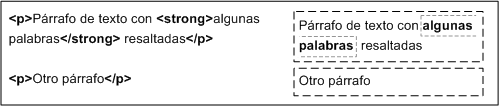
\includegraphics[width=0.8\textwidth]{img/f0402.png}
\end{figure}
\end{center}

\end{frame}

%%---------------------------------------------------------------

\begin{frame}
\frametitle{El modelo de cajas (II)}

\begin{itemize}
  \item No son visibles a simple vista porque inicialmente no muestran ningún color de fondo ni ningún borde
\end{itemize}

\begin{center}
\begin{figure}[p]
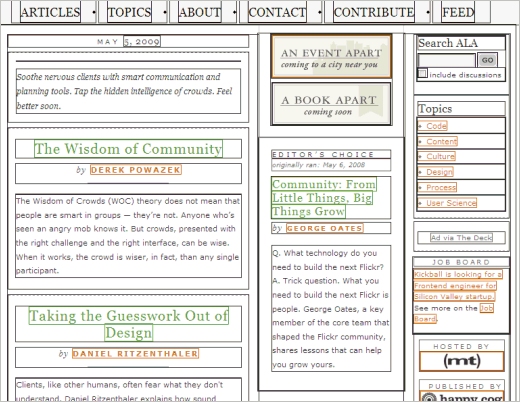
\includegraphics[width=0.55\textwidth]{img/f0401.png}
\end{figure}
\end{center}
{\footnotesize
Ejemplo de http://www.alistapart.com/ después de forzar a que todas las cajas muestren su borde
}

\end{frame}

%%---------------------------------------------------------------

\begin{frame}
\frametitle{El modelo de cajas (III)}

\begin{itemize}
  \item Los navegadores crean y colocan las cajas de forma automática, pero CSS permite modificar todas sus características. Cada una de las cajas está formada por seis partes, tal y como muestra la siguiente imagen:
\end{itemize}


\begin{center}
\begin{figure}[p]
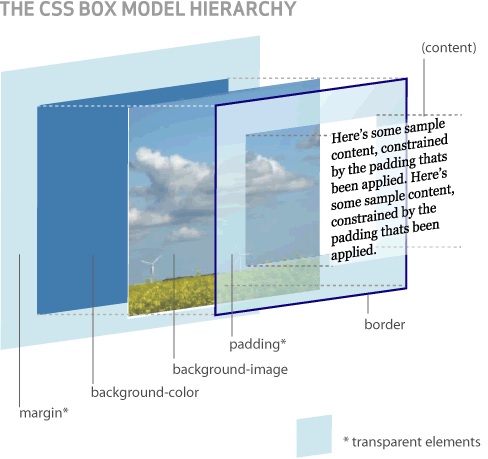
\includegraphics[width=0.45\textwidth]{img/f0403.png}
\end{figure}
\end{center}
{\footnotesize
 Representación tridimensional del box model de CSS
(Esquema utilizado con permiso de http://www.hicksdesign.co.uk/boxmodel/)
}
\end{frame}

%%---------------------------------------------------------------

\begin{frame}
\frametitle{Partes que componen cada caja}

\begin{itemize}
  \item Contenido (content): se trata del contenido HTML del elemento (las palabras de un párrafo, una imagen, el texto de una lista de elementos, etc.)
  \item Relleno (padding): espacio libre opcional existente entre el contenido y el borde.
  \item Borde (border): línea que encierra completamente el contenido y su relleno.
  \item Imagen de fondo (background image): imagen que se muestra por detrás del contenido y el espacio de relleno.
  \item Color de fondo (background color): color que se muestra por detrás del contenido y el espacio de relleno.
  \item Margen (margin): separación opcional existente entre la caja y el resto de cajas adyacentes.
\end{itemize}

\end{frame}

%%---------------------------------------------------------------

\begin{frame}
\frametitle{Orden de visualización}

\begin{itemize}
  \item El relleno y el margen son transparentes, por lo que en el espacio ocupado por el relleno se muestra el color o imagen de fondo (si están definidos)
  \item En el espacio ocupado por el margen se muestra el color o imagen de fondo de su elemento padre (si están definidos)
  \item Si ningún elemento padre tiene definido un color o imagen de fondo, se muestra el color o imagen de fondo de la propia página (si están definidos)
  \item Si una caja define tanto un color como una imagen de fondo, la imagen tiene más prioridad y es la que se visualiza
  \item Si la imagen de fondo no cubre totalmente la caja del elemento o si la imagen tiene zonas transparentes, también se visualiza el color de fondo. 
\end{itemize}

\end{frame}

%%---------------------------------------------------------------

\begin{frame}
\frametitle{Propiedad width}

\begin{center}
  \begin{table}
   \begin{tabular}{p{1.8cm}p{7.8cm}}
Propiedad &\bf{width} \\ \hline
Valores & $<medida>$ | $<porcentaje>$ | auto | inherit \\ \hline
Se aplica a & Todos los elementos, salvo los elementos en línea que no sean imágenes, las filas de tabla y los grupos de filas de tabla \\ \hline
Valor inicial & auto \\ \hline
Descripción & Establece la anchura de un elemento \\ \hline
  \end{tabular}
   \caption{Definición de la propiedad width de CSS}
 \end{table}
\end{center}

\end{frame}

%%---------------------------------------------------------------

\begin{frame}
\frametitle{Propiedad height}

\begin{center}
  \begin{table}
   \begin{tabular}{p{1.8cm}p{7.8cm}}
Propiedad &\bf{height} \\ \hline
Valores & $<medida>$ | $<porcentaje>$ | auto | inherit \\ \hline
Se aplica a & Todos los elementos, salvo los elementos en línea que no sean imágenes, las columnas de tabla y los grupos de columnas de tabla \\ \hline
Valor inicial & auto \\ \hline
Descripción & Establece la altura de un elemento \\ \hline
  \end{tabular}
   \caption{Definición de la propiedad height de CSS}
 \end{table}
\end{center}

\end{frame}

%%---------------------------------------------------------------

\begin{frame}
\frametitle{Propiedades margin}

\begin{center}
  \begin{table}
   \begin{tabular}{p{1.8cm}p{7.8cm}}
Propiedades &\bf{margin-top}, \bf{margin-right}, \bf{margin-bottom}, \bf{margin-left} \\ \hline
Valores & $<medida>$ | $<porcentaje>$ | auto | inherit \\ \hline
Se aplica a & Todos los elementos, salvo margin-top y margin-bottom que sólo se aplican a los elementos de bloque y a las imágenes \\ \hline
Valor inicial & 0 \\ \hline
Descripción & Establece cada uno de los márgenes horizontales y verticales de un elemento \\  \hline
  \end{tabular}
    \caption{Definición de la propiedad margin-top, margin-right, margin-bottom, margin-left de CSS}
 \end{table}
\end{center}

\end{frame}

%%---------------------------------------------------------------

\begin{frame}
\frametitle{Márgenes}


\begin{center}
\begin{figure}[p]
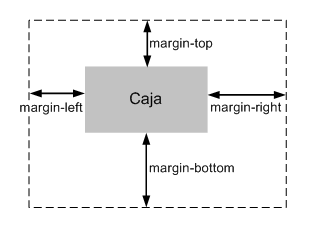
\includegraphics[width=0.45\textwidth]{img/f0428.png}
\end{figure}
\end{center}

\begin{itemize}
  \item En vez de utilizar la etiqueta <blockquote> de HTML, debería utilizarse la propiedad margin-left de CS
  \item Los márgenes verticales (margin-top y margin-bottom) sólo se pueden aplicar a los elementos de bloque y las imágenes, mientras que los márgenes laterales (margin-left y margin-right) se pueden aplicar a cualquier elemento
\end{itemize}

\end{frame}

%%---------------------------------------------------------------

\begin{frame}
\frametitle{Propiedad margin (propiedad \emph{shorthand})}

\begin{center}
  \begin{table}
   \begin{tabular}{p{1.8cm}p{7.8cm}}
Propiedad &\bf{margin} \\ \hline
Valores & ( $<medida>$ | $<porcentaje>$ | auto ) {1, 4} | inherit \\ \hline
Se aplica a & Todos los elementos salvo algunos casos especiales de elementos mostrados como tablas \\ \hline
Valor inicial & - \\ \hline
Descripción & Establece de forma directa todos los márgenes de un elemento \\ \hline
 \end{tabular}
   \caption{Definición de la propiedad margin de CSS}
 \end{table}
\end{center}

\end{frame}

%%---------------------------------------------------------------

\begin{frame}
\frametitle{Propiedad margin (propiedad \emph{shorthand}) (y II)}

La notación {1, 4} de la definición anterior significa que la propiedad margin admite entre uno y cuatro valores, con el siguiente significado:

\begin{itemize}
  \item Si solo se indica un valor, todos los márgenes tienen ese valor.
  \item Si se indican dos valores, el primero se asigna al margen superior e inferior y el segundo se asigna a los márgenes izquierdo y derecho.
  \item Si se indican tres valores, el primero se asigna al margen superior, el tercero se asigna al margen inferior y el segundo valor se asigna los márgenes izquierdo y derecho.
  \item Si se indican los cuatro valores, el orden de asignación es: margen superior, margen derecho, margen inferior y margen izquierdo.
\end{itemize}

\end{frame}

%%---------------------------------------------------------------

\begin{frame}
\frametitle{El margen vertical}

Es algo peculiar:

\begin{itemize}
  \item Cuando se juntan dos o más márgenes verticales, se fusionan de forma automática y la altura del nuevo margen será igual a la altura del margen más alto de los que se han fusionado.
  \item Si un elemento está contenido dentro de otro elemento, sus márgenes verticales se fusionan y resultan en un nuevo margen de la misma altura que el mayor margen de los que se han fusionado
  \item Si no se diera este comportamiento y se estableciera un determinado margen a todos los párrafos, el primer párrafo no mostraría un aspecto homogéneo respecto de los demás.
\end{itemize}

\end{frame}

%%---------------------------------------------------------------

\begin{frame}
\frametitle{Relleno}

\begin{center}
  \begin{table}
   \begin{tabular}{p{1.8cm}p{7.8cm}}
Propiedades &\bf{padding-top}, \bf{padding-right}, \bf{padding-bottom}, \bf{padding-left} \\ \hline
Valores & $<medida>$ | $<porcentaje>$ | inherit \\ \hline
Se aplica a & Todos los elementos excepto algunos elementos de tablas como grupos de cabeceras y grupos de pies de tabla \\ \hline
Valor inicial & 0 \\ \hline
Descripción & Establece cada uno de los rellenos horizontales y verticales de un elemento \\ \hline
  \end{tabular}
   \caption{Definición de la propiedad padding-top, padding-right, padding-bottom, padding-left de CSS}
 \end{table}
\end{center}

\end{frame}

%%---------------------------------------------------------------

\begin{frame}
\frametitle{}

\begin{center}
  \begin{table}
   \begin{tabular}{p{1.8cm}p{7.8cm}}
Propiedad &\bf{padding} \\ \hline
Valores & ( $<medida>$ | $<porcentaje>$ ) {1, 4} | inherit \\ \hline
Se aplica a & Todos los elementos excepto algunos elementos de tablas como grupos de cabeceras y grupos de pies de tabla \\ \hline
Valor inicial & - \\ \hline
Descripción & Establece de forma directa todos los rellenos de los elementos \\ \hline
  \end{tabular}
   \caption{Definición de la propiedad padding de CSS}
 \end{table}
\end{center}

\end{frame}

%%---------------------------------------------------------------

\begin{frame}
\frametitle{Anchura de los bordes}

\begin{center}
  \begin{table}
   \begin{tabular}{p{1.8cm}p{7.8cm}}
Propiedades &\bf{border-top-width}, \bf{border-right-width}, \bf{border-bottom-width}, \bf{border-left-width} \\ \hline
Valores & ( $<medida>$ | thin | medium | thick ) | inherit \\ \hline
Se aplica a & Todos los elementos \\ \hline
Valor inicial & Medium \\ \hline
Descripción & Establece la anchura de cada uno de los cuatro bordes de los elementos \\ \hline
  \end{tabular}
   \caption{Definición de la propiedad border-top-width, border-right-width, border-bottom-width, border-left-width de CSS}
 \end{table}
\end{center}

\end{frame}

%%---------------------------------------------------------------

\begin{frame}
\frametitle{Anchura de los bordes (shorthand)}

\begin{center}
  \begin{table}
   \begin{tabular}{p{1.8cm}p{7.8cm}}
Propiedad &\bf{border-width} \\ \hline
Valores & ( $<medida>$ | thin | medium | thick ) {1, 4} | inherit \\ \hline
Se aplica a & Todos los elementos \\ \hline
Valor inicial & Medium \\ \hline
Descripción & Establece la anchura de todos los bordes del elemento \\ \hline
  \end{tabular}
   \caption{Definición de la propiedad border-width de CSS}
 \end{table}
\end{center}

\end{frame}

%%---------------------------------------------------------------

\begin{frame}
\frametitle{Color de los bordes}

\begin{center}
  \begin{table}
   \begin{tabular}{p{1.8cm}p{7.8cm}}
Propiedades & \bf{border-top-color}, \bf{border-right-color}, \bf{border-bottom-color}, \bf{border-left-color} \\ \hline
Valores & $<color>$ | transparent | inherit \\ \hline
Se aplica a & Todos los elementos \\ \hline
Valor inicial & - \\ \hline
Descripción & Establece el color de cada uno de los cuatro bordes de los elementos \\ \hline
  \end{tabular}
   \caption{Definición de la propiedad border-top-color, border-right-color, border-bottom-color, border-left-color de CSS}
 \end{table}
\end{center}

\end{frame}

%%---------------------------------------------------------------

\begin{frame}
\frametitle{Color de los bordes (shorthand)}

\begin{center}
  \begin{table}
   \begin{tabular}{p{1.8cm}p{7.8cm}}
Propiedad &\bf{border-color} \\ \hline
Valores & ( $<color>$ | transparent ) {1, 4} | inherit \\ \hline
Se aplica a & Todos los elementos \\ \hline
Valor inicial & - \\ \hline
Descripción & Establece el color de todos los bordes del elemento \\ \hline
  \end{tabular}
   \caption{Definición de la propiedad border-color de CSS}
 \end{table}
\end{center}

\end{frame}

%%---------------------------------------------------------------

\begin{frame}
\frametitle{Estilo de los bordes}

\begin{center}
  \begin{table}
   \begin{tabular}{p{1.8cm}p{7.8cm}}
Propiedades &\bf{border-top-style}, \bf{border-right-style}, \bf{border-bottom-style}, \bf{border-left-style} \\ \hline
Valores & none | hidden | dotted | dashed | solid | double | groove | ridge | inset | outset | inherit \\ \hline
Se aplica a & Todos los elementos \\ \hline
Valor inicial & none \\ \hline
Descripción & Establece el estilo de cada uno de los cuatro bordes de los elementos \\ \hline
  \end{tabular}
   \caption{Definición de la propiedad border-top-style, border-right-style, border-bottom-style, border-left-style de CSS}
 \end{table}
\end{center}

\end{frame}

%%---------------------------------------------------------------

\begin{frame}
\frametitle{Estilo de los bordes \emph{shorthand}}

\begin{center}
  \begin{table}
   \begin{tabular}{p{1.8cm}p{7.8cm}}
Propiedad &\bf{border-style} \\ \hline
Valores & (none | hidden | dotted | dashed | solid | double | groove | ridge | inset | outset ) {1, 4} | inherit \\ \hline
Se aplica a & Todos los elementos \\ \hline
Valor inicial & - \\ \hline
Descripción & Establece el estilo de todos los bordes del elemento \\ \hline
  \end{tabular}
   \caption{Definición de la propiedad border-style de CSS}
 \end{table}
\end{center}

\end{frame}

%%---------------------------------------------------------------

\begin{frame}
\frametitle{Propiedades \emph{shorthand} para bordes}

\begin{center}
  \begin{table}
   \begin{tabular}{p{1.8cm}p{7.8cm}}
Propiedades &\bf{border-top}, \bf{border-right}, \bf{border-bottom}, \bf{border-left} \\ \hline
Valores & ( $<medida\_borde>$ || $<color\_borde>$ || $<estilo\_borde>$ ) | inherit \\ \hline
Se aplica a & Todos los elementos \\ \hline
Valor inicial & - \\ \hline
Descripción & Establece el estilo completo de cada uno de los cuatro bordes de los elementos \\ \hline
 \end{tabular}
   \caption{Definición de la propiedad border-top, border-right, border-bottom, border-left de CSS}
 \end{table}
\end{center}

\end{frame}

%%---------------------------------------------------------------

\begin{frame}
\frametitle{Propiedad shorthand para borde (global)}

\begin{center}
  \begin{table}
   \begin{tabular}{p{1.8cm}p{7.8cm}}
Propiedad &\bf{border} \\ \hline
Valores & ( $<medida\_borde>$ || $<color\_borde>$ || $<estilo\_borde>$ ) | inherit \\ \hline
Se aplica a & Todos los elementos \\ \hline
Valor inicial & - \\ \hline
Descripción & Establece el estilo completo de todos los bordes de los elementos \\ \hline
 \end{tabular}
   \caption{Definición de la propiedad border de CSS}
 \end{table}
\end{center}

\end{frame}

%%---------------------------------------------------------------

\begin{frame}[fragile]
\frametitle{Más sobre bordes}

\begin{itemize}
  \item Como el valor por defecto de la propiedad border-style es none, si una propiedad shorthand no establece explícitamente el estilo de un borde, el elemento no muestra ese borde
  \item Cuando los cuatro bordes no son idénticos pero sí muy parecidos, se puede utilizar la propiedad border para establecer de forma directa los atributos comunes de todos los bordes y posteriormente especificar para cada uno de los cuatro bordes sus propiedades particulares:
\begin{verbatim}
h1 {
  border: solid #000;
  border-top-width: 6px;
  border-left-width: 8px;
}
\end{verbatim}
\end{itemize}

\end{frame}

%%---------------------------------------------------------------

\begin{frame}[fragile]
\frametitle{Margen, relleno, bordes y modelo de cajas (I)}

\begin{itemize}
  \item El margen, el relleno y los bordes establecidos a un elemento determinan la anchura y altura final del elemento
\end{itemize}

{\footnotesize
\begin{verbatim}
div {
  width: 300px;
  padding-left:  50px;
  padding-right: 50px;
  margin-left:   30px;
  margin-right:  30px;
  border: 10px solid black;
}
\end{verbatim}
}



\end{frame}

%%---------------------------------------------------------------

\begin{frame}[fragile]
\frametitle{Margen, relleno, bordes y modelo de cajas (y II)}

\begin{center}
\begin{figure}[p]
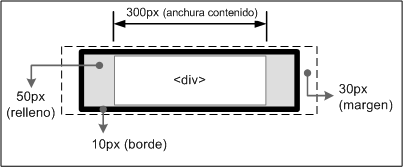
\includegraphics[width=0.75\textwidth]{img/f0414.png}
\end{figure}
\end{center}

De esta forma, la anchura del elemento en pantalla sería igual a la suma de la anchura original, los márgenes, los bordes y los rellenos:

30px + 10px + 50px + 300px + 50px + 10px + 30px = 480 píxel

\end{frame}

%%---------------------------------------------------------------

\begin{frame}
\frametitle{Fondos}

\begin{itemize}
  \item Puede ser un color simple o una imagen.
  \item Solamente se visualiza en el área ocupada por el contenido y su relleno, ya que el color de los bordes se controla directamente desde los bordes y las zonas de los márgenes siempre son transparentes
  \item Se puede establecer de forma simultánea un color y una imagen de fondo. En este caso, la imagen se muestra delante del color, por lo que solamente si la imagen contiene zonas transparentes es posible ver el color de fondo.
\end{itemize}

\end{frame}


%%---------------------------------------------------------------

\begin{frame}
\frametitle{Propiedad background-color}

\begin{center}
  \begin{table}
   \begin{tabular}{p{1.8cm}p{7.8cm}}
Propiedad & \bf{background-color} \\ \hline
Valores& $color>$ | transparent | inherit \\ \hline
Se aplica a& Todos los elementos \\ \hline
Valor inicial& transparent \\ \hline
Descripción& Establece un color de fondo para los elementos \\ \hline
  \end{tabular}
   \caption{Definición de la propiedad background-color de CSS}
 \end{table}
\end{center}


\end{frame}


%%---------------------------------------------------------------

\begin{frame}
\frametitle{Propiedad background-image}

\begin{center}
  \begin{table}
   \begin{tabular}{p{1.8cm}p{7.8cm}}
Propiedad & \bf{background-image} \\ \hline
Valores& $url>$ | none | inherit \\ \hline
Se aplica a& Todos los elementos \\ \hline
Valor inicial& none \\ \hline
Descripción& Establece una imagen como fondo para los elementos \\ \hline
  \end{tabular}
   \caption{Definición de la propiedad background-image de CSS}
 \end{table}
\end{center}


\end{frame}


%%---------------------------------------------------------------

\begin{frame}
\frametitle{Propiedad background-repeat}

\begin{center}
  \begin{table}
   \begin{tabular}{p{1.8cm}p{7.8cm}}
Propiedad & \bf{background-repeat} \\ \hline
Valores& repeat | repeat-x | repeat-y | no-repeat | inherit \\ \hline
Se aplica a& Todos los elementos \\ \hline
Valor inicial& repeat \\ \hline
Descripción& Controla la forma en la que se repiten las imágenes de fondo \\ \hline
  \end{tabular}
   \caption{Definición de la propiedad background-repeat de CSS}
 \end{table}
\end{center}


\end{frame}


%%---------------------------------------------------------------

\begin{frame}
\frametitle{Propiedad background-position}

\begin{center}
  \begin{table}
   \begin{tabular}{p{1.8cm}p{7.8cm}}
Propiedad & \bf{background-position} \\ \hline
Valores& ( ( $<porcentaje>$ | $<medida>$ | left | center | right ) ( $<porcentaje>$ | $<medida>$ | top | center | bottom )? ) | ( ( left | center | right ) || ( top | center | bottom ) ) | inherit \\ \hline
Se aplica a& Todos los elementos \\ \hline
Valor inicial& 0\% 0\% \\ \hline
Descripción& Controla la posición en la que se muestra la imagen en el fondo del elemento \\ \hline
  \end{tabular}
   \caption{Definición de la propiedad background-position de CSS}
 \end{table}
\end{center}


\end{frame}


%%---------------------------------------------------------------

\begin{frame}
\frametitle{Propiedad background-attachment}

\begin{center}
  \begin{table}
   \begin{tabular}{p{1.8cm}p{7.8cm}}
Propiedad & \bf{background-attachment} \\ \hline
Valores& scroll | fixed | inherit \\ \hline
Se aplica a& Todos los elementos \\ \hline
Valor inicial& scroll \\ \hline
Descripción& Controla la forma en la que se visualiza la imagen de fondo: permanece fija cuando se hace scroll en la ventana del navegador o se desplaza junto con la ventana \\ \hline
  \end{tabular}
   \caption{Definición de la propiedad background-attachment de CSS}
 \end{table}
\end{center}


\end{frame}


%%---------------------------------------------------------------

\begin{frame}
\frametitle{Propiedad ''shorthand" background}

\begin{center}
  \begin{table}
   \begin{tabular}{p{1.8cm}p{7.8cm}}
Propiedad & \bf{background} \\ \hline
Valores& ( $background-color$ || $background-image$ || $background-repeat$ || $background-attachment$ || $background-position$ ) | inherit \\ \hline
Se aplica a& Todos los elementos \\ \hline
Valor inicial& - \\ \hline
Descripción& Establece todas las propiedades del fondo de un elemento \\ \hline
  \end{tabular}
   \caption{Definición de la propiedad background de CSS}
 \end{table}
\end{center}


\end{frame}



%%---------------------------------------------------------------
\section{Posicionamiento y visualización}

\begin{frame}
\frametitle{Posicionamiento y visualización}

\begin{itemize}
  \item Cuando los navegadores descargan el contenido HTML y CSS de las páginas web, aplican un procesamiento muy complejo antes de mostrar las páginas en la pantalla del usuario
  \item Para cumplir con el modelo de cajas, los navegadores crean una caja para representar a cada elemento de la página HTML.
  \item Existen cinco tipos de posicionamientos definidos para las cajas y se presentan otras propiedades que afectan a la forma en la que se visualizan las cajas.
\end{itemize}

\end{frame}


%%---------------------------------------------------------------

\begin{frame}
\frametitle{Tipos de elementos (I)}

El estándar HTML clasifica a todos sus elementos en dos grandes grupos:

Elementos de línea:

\begin{itemize}
  \item Los elementos en línea ("inline elements" en inglés) no empiezan necesariamente en nueva línea y sólo ocupan el espacio necesario para mostrar sus contenidos.

\end{itemize}

\end{frame}

%%---------------------------------------------------------------

\begin{frame}
\frametitle{Tipos de elementos (II)}

Elementos de bloque:

\begin{itemize}
  \item Los elementos de bloque ("block elements" en inglés) siempre empiezan en una nueva línea y ocupan todo el espacio disponible hasta el final de la línea
\end{itemize}

\begin{center}
\begin{figure}[p]
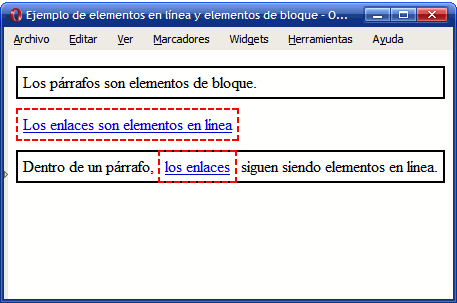
\includegraphics[width=0.8\textwidth]{img/f0501.png}
\end{figure}
\end{center}

Por sus características, los elementos de bloque no pueden insertarse dentro de elementos en línea y tan sólo pueden aparecer dentro de otros elementos de bloque. En cambio, un elemento en línea puede aparecer tanto dentro de un elemento de bloque como dentro de otro elemento en línea.

\end{frame}


%%---------------------------------------------------------------

\begin{frame}
\frametitle{Posicionamiento}

\begin{itemize}
  \item Los navegadores crean y posicionan de forma automática todas las cajas que forman cada página HTML
  \item El diseñador puede modificar la posición en la que se muestra cada caja.
  \item Existen 4 tipos de posicionamiento diferente
\end{itemize}

\end{frame}


%%---------------------------------------------------------------

\begin{frame}
\frametitle{Tipos de posicionamiento}

\begin{itemize}
  \item Posicionamiento normal o estático: posicionamientosi no se indica lo contrario.
  \item Posicionamiento relativo: consiste en posicionar una caja según el posicionamiento normal y después desplazarla respecto de su posición original.
  \item Posicionamiento absoluto: la posición de una caja se establece de forma absoluta respecto de su elemento contenedor y el resto de elementos de la página ignoran la nueva posición del elemento.
  \item Posicionamiento fijo: variante del posicionamiento absoluto que convierte una caja en un elemento inamovible, de forma que su posición en la pantalla siempre es la misma independientemente del resto de elementos e independientemente de si el usuario sube o baja la página en la ventana del navegador.
  \item Posicionamiento flotante: desplaza las cajas todo lo posible hacia la izquierda o hacia la derecha de la línea en la que se encuentran.
\end{itemize}

\end{frame}


%%---------------------------------------------------------------

\begin{frame}
\frametitle{Propiedad position}

\begin{center}
  \begin{table}
   \begin{tabular}{p{1.8cm}p{7.8cm}}
Propiedad & \bf{position} \\ \hline
Valores& static | relative | absolute | fixed | inherit \\ \hline
Se aplica a& Todos los elementos \\ \hline
Valor inicial& static \\ \hline
Descripción& Selecciona el posicionamiento con el que se mostrará el elemento \\ \hline
  \end{tabular}
   \caption{Definición de la propiedad position de CSS}
 \end{table}
\end{center}


\end{frame}


%%---------------------------------------------------------------

\begin{frame}
\frametitle{Significados propiedad position}

\begin{itemize}
  \item static: corresponde al posicionamiento normal o estático. Si se utiliza este valor, se ignoran los valores de las propiedades top, right, bottom y left que se verán a continuación.
  \item relative: corresponde al posicionamiento relativo. El desplazamiento de la caja se controla con las propiedades top, right, bottom y left.
  \item absolute: corresponde al posicionamiento absoluto. El desplazamiento de la caja también se controla con las propiedades top, right, bottom y left, pero su interpretación es mucho más compleja, ya que el origen de coordenadas del desplazamiento depende del posicionamiento de su elemento contenedor.
  \item fixed: corresponde al posicionamiento fijo. El desplazamiento se establece de la misma forma que en el posicionamiento absoluto, pero en este caso el elemento permanece inamovible en la pantalla.
\end{itemize}

\end{frame}


%%---------------------------------------------------------------

\begin{frame}
\frametitle{Propiedades top, right, bottom, left}

\begin{center}
  \begin{table}
   \begin{tabular}{p{1.8cm}p{7.8cm}}
Propiedades& {\bf top}, {\bf right}, {\bf bottom}, {\bf left} \\ \hline
Valores& $<medida>$ | $<porcentaje>$ | auto | inherit \\ \hline
Se aplica a& Todos los elementos posicionados \\ \hline
Valor inicial& auto \\ \hline
Descripción& Indican el desplazamiento horizontal y vertical del elemento respecto de su posición original \\ \hline
  \end{tabular}
   \caption{Definición de la propiedad top, right, bottom, left de CSS}
 \end{table}
\end{center}


\end{frame}


%%---------------------------------------------------------------

\begin{frame}
\frametitle{Posicionamiento normal (o estático)}

\begin{itemize}
  \item Utilizado por defecto por los navegadores
  \item Sólo se tiene en cuenta si el elemento es de bloque o en línea, sus propiedades width y height y su contenido.
  \item Las cajas se muestran una debajo de otra comenzando desde el principio del elemento contenedor. La distancia entre las cajas se controla mediante los márgenes verticales.
  \item Si un elemento se encuentra dentro de otro, el elemento padre se llama "elemento contenedor" y determina tanto la posición como el tamaño de todas sus cajas interiores.
\end{itemize}


\begin{center}
\begin{figure}[p]
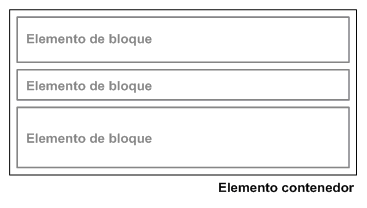
\includegraphics[width=0.8\textwidth]{img/f0502.png}
\end{figure}
\end{center}

\end{frame}


%%---------------------------------------------------------------

\begin{frame}
\frametitle{Posicionamiento normal (o estático) (y II)}

\begin{itemize}
  \item Los elementos en línea forman los "contextos de formato en línea". Las cajas se muestran una detrás de otra de forma horizontal comenzando desde la posición más a la izquierda de su elemento contenedor.
  \item Si las cajas en línea ocupan más espacio del disponible en su propia línea, el resto de cajas se muestran en las líneas inferiores. 
  \item Si las cajas en línea ocupan un espacio menor que su propia línea, se puede controlar la distribución de las cajas mediante la propiedad text-align para centrarlas, alinearlas a la derecha o justificarlas.
\end{itemize}


\begin{center}
\begin{figure}[p]
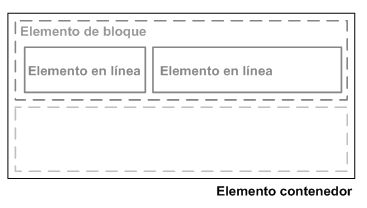
\includegraphics[width=0.8\textwidth]{img/f0503.png}
\end{figure}
\end{center}

\end{frame}


%%---------------------------------------------------------------

\begin{frame}
\frametitle{Posicionamiento relativo}

\begin{itemize}
  \item Desplaza una caja respecto de su posición original establecida mediante el posicionamiento normal. El desplazamiento de la caja se controla con las propiedades top, right, bottom y left.
  \item la propiedad top se emplea para mover las cajas de forma descendente, la propiedad bottom mueve las cajas de forma ascendente, la propiedad left se utiliza para desplazar las cajas hacia la derecha y la propiedad right mueve las cajas hacia la izquierda. 
\end{itemize}

\begin{center}
\begin{figure}[p]
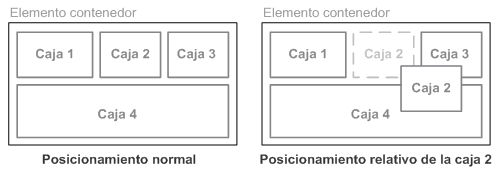
\includegraphics[width=0.8\textwidth]{img/f0504.png}
\end{figure}
\end{center}

\end{frame}


%%---------------------------------------------------------------

\begin{frame}
\frametitle{Posicionamiento absoluto}

\begin{itemize}
  \item Se emplea para establecer de forma exacta la posición en la que se muestra la caja de un elemento. 
  \item Cuando una caja se posiciona de forma absoluta, el resto de elementos de la página se ven afectados y modifican su posición. 
\end{itemize}

\begin{center}
\begin{figure}[p]
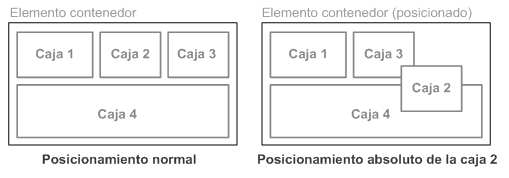
\includegraphics[width=0.8\textwidth]{img/f0516.png}
\end{figure}
\end{center}

\end{frame}


%%---------------------------------------------------------------

\begin{frame}
\frametitle{Posicionamiento absoluto}

\begin{itemize}
  \item El primer elemento contenedor que esté posicionado de cualquier forma diferente a position: static se convierte en la referencia que determina la posición de la caja posicionada de forma absoluta.
  \item Si ningún elemento contenedor está posicionado, la referencia es la ventana del navegador, que no debe confundirse con el elemento $<body>$ de la página.
  \item Una vez determinada la referencia del posicionamiento absoluto, la interpretación de los valores de las propiedades top, right, bottom y left se realiza como sigue:
  \begin{itemize}
    \item Top: desplazamiento desde el borde superior del elemento contenedor que se utiliza como referencia.
    \item Right: ídem pero desde el borde derecho al borde derecho.
    \item Left:  ídem pero desde el borde izquierdo al borde izquierdo.
    \item Bottom: ídem pero desde el borde inferior al borde inferior.
  \end{itemize}
\end{itemize}

\end{frame}


%%---------------------------------------------------------------

\begin{frame}
\frametitle{Diferencias entre posicionamiento absoluto y relativo}

\begin{center}
\begin{figure}[p]
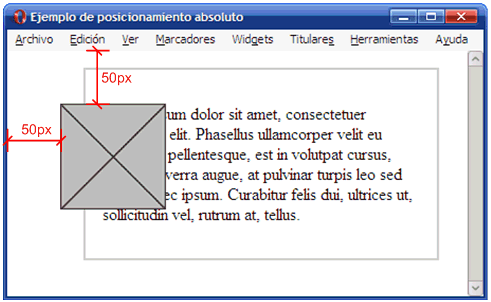
\includegraphics[width=0.6\textwidth]{img/f0519.png}
\end{figure}
\end{center}

\begin{center}
\begin{figure}[p]
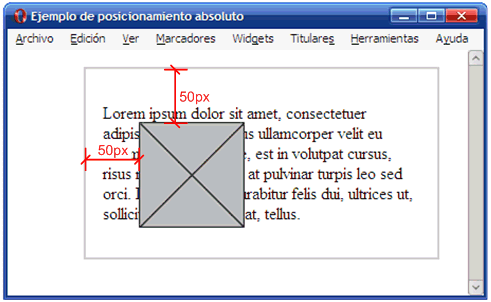
\includegraphics[width=0.6\textwidth]{img/f0521.png}
\end{figure}
\end{center}

\end{frame}


%%---------------------------------------------------------------

\begin{frame}
\frametitle{Posicionamiento fijo}

\begin{itemize}
  \item Es un caso particular del posicionamiento absoluto, ya que sólo se diferencian en el comportamiento de las cajas posicionadas.
  \item La principal característica de una caja posicionada de forma fija es que su posición es inamovible dentro de la ventana del navegador.
  \item El posicionamiento fijo hace que las cajas no modifiquen su posición ni aunque el usuario suba o baje la página en la ventana de su navegador.
  \item Si la página se visualiza en un medio paginado (por ejemplo en una impresora) las cajas posicionadas de forma fija se repiten en todas las páginas.
\end{itemize}

\end{frame}


%%---------------------------------------------------------------

\begin{frame}
\frametitle{Posicionamiento flotante}

\begin{itemize}
  \item Cuando una caja se posiciona con el modelo de posicionamiento flotante, automáticamente se convierte en una caja flotante, lo que significa que se desplaza hasta la zona más a la izquierda o más a la derecha de la posición en la que originalmente se encontraba.
\end{itemize}


\begin{center}
\begin{figure}[p]
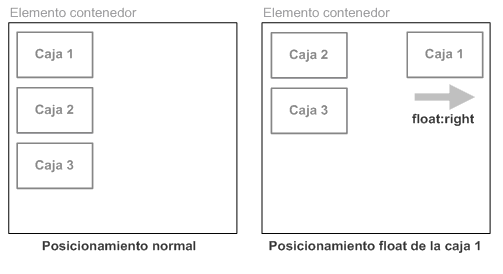
\includegraphics[width=0.8\textwidth]{img/f0507.png}
\end{figure}
\end{center}

\end{frame}


%%---------------------------------------------------------------

\begin{frame}
\frametitle{Posicionamiento flotante (y II)}

\begin{itemize}
  \item Cuando se posiciona una caja de forma flotante:
  \begin{itemize}
    \item La caja deja de pertenecer al flujo normal de la página, lo que significa que el resto de cajas ocupan el lugar dejado por la caja flotante.
    \item La caja flotante se posiciona lo más a la izquierda o lo más a la derecha posible de la posición en la que se encontraba originalmente.
  \end{itemize}
\end{itemize}


\begin{center}
\begin{figure}[p]
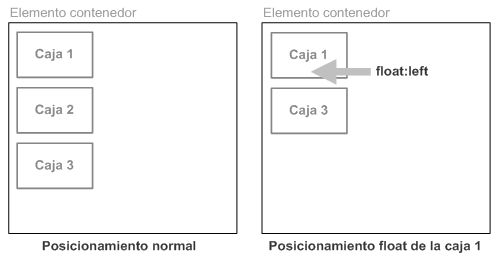
\includegraphics[width=0.8\textwidth]{img/f0508.png}
\end{figure}
\end{center}

\end{frame}


%%---------------------------------------------------------------

\begin{frame}
\frametitle{Posicionamiento flotante (y III)}

\begin{itemize}
  \item Si existen otras cajas flotantes, al posicionar de forma flotante otra caja, se tiene en cuenta el sitio disponible.
  \item Si no existiera sitio en la línea actual, la caja flotante baja a la línea inferior hasta que encuentra el sitio necesario para mostrarse lo más a la izquierda o lo más a la derecha posible en esa nueva línea
\end{itemize}


\begin{center}
\begin{figure}[p]
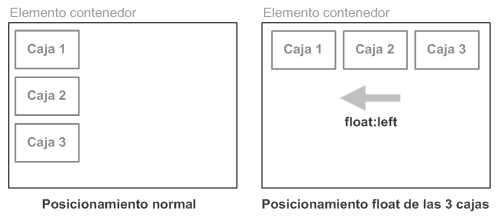
\includegraphics[width=0.8\textwidth]{img/f0509.png}
\end{figure}
\end{center}

\end{frame}


%%---------------------------------------------------------------

\begin{frame}
\frametitle{Propiedad float}

\begin{center}
  \begin{table}
   \begin{tabular}{p{1.8cm}p{7.8cm}}
Propiedad & \bf{float} \\ \hline
Valores& left | right | none | inherit \\ \hline
Se aplica a& Todos los elementos \\ \hline
Valor inicial& none \\ \hline
Descripción& Establece el tipo de posicionamiento flotante del elemento \\ \hline
  \end{tabular}
   \caption{Definición de la propiedad float de CSS}
 \end{table}
\end{center}


\end{frame}


%%---------------------------------------------------------------

\begin{frame}
\frametitle{Posicionamiento flotante (y IV)}

\begin{itemize}
  \item Los elementos que se encuentran alrededor de una caja flotante adaptan sus contenidos para que fluyan alrededor del elemento posicionado
  \item Uno de los principales motivos para la creación del posicionamiento float fue precisamente la posibilidad de colocar imágenes alrededor de las cuales fluye el texto.
\end{itemize}


\begin{center}
\begin{figure}[p]
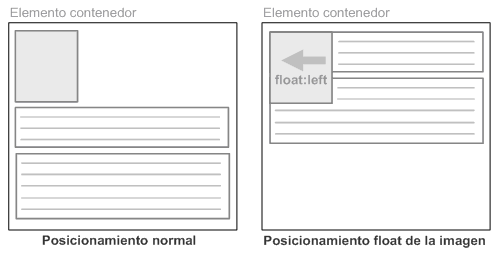
\includegraphics[width=0.8\textwidth]{img/f0513.png}
\end{figure}
\end{center}

\end{frame}


%%---------------------------------------------------------------

\begin{frame}
\frametitle{Propiedad clear}

\begin{itemize}
  \item La propiedad clear indica el lado del elemento HTML que no debe ser adyacente a ninguna caja posicionada de forma flotante. Si se indica el valor left, el elemento se desplaza de forma descendente hasta que pueda colocarse en una línea en la que no haya ninguna caja flotante en el lado izquierdo.
  \item La especificación oficial de CSS explica este comportamiento como "un desplazamiento descendente hasta que el borde superior del elemento esté por debajo del borde inferior de cualquier elemento flotante hacia la izquierda".
\end{itemize}

\end{frame}


%%---------------------------------------------------------------

\begin{frame}
\frametitle{Propiedad clear}

\begin{center}
  \begin{table}
   \begin{tabular}{p{1.8cm}p{7.8cm}}
Propiedad & \bf{clear} \\ \hline
Valores& none | left | right | both | inherit \\ \hline
Se aplica a& Todos los elementos de bloque \\ \hline
Valor inicial& none \\ \hline
Descripción& Indica el lado del elemento que no debe ser adyacente a ninguna caja flotante \\ \hline
  \end{tabular}
   \caption{Definición de la propiedad clear de CSS}
 \end{table}
\end{center}


\end{frame}


%%---------------------------------------------------------------

\begin{frame}
\frametitle{Visualización}

\begin{itemize}
  \item CSS define otras cuatro propiedades para controlar su visualización: display, visibility, overflow y z-index.
  \item La propiedad display permite ocultar completamente un elemento haciendo que desaparezca de la página. Como el elemento oculto no se muestra, el resto de elementos de la página se mueven para ocupar su lugar.
  \item La propiedad display también permite modificar el comportamiento de un elemento a bloque (block) o en línea (inline).
  \item La propiedad visibility permite hacer invisible un elemento, lo que significa que el navegador crea la caja del elemento pero no la muestra. En este caso, el resto de elementos de la página no modifican su posición, ya que aunque la caja no se ve, sigue ocupando sitio.
\end{itemize}

\end{frame}


%%---------------------------------------------------------------

\begin{frame}
\frametitle{Diferencias entre display y visibility}

\begin{center}
\begin{figure}[p]
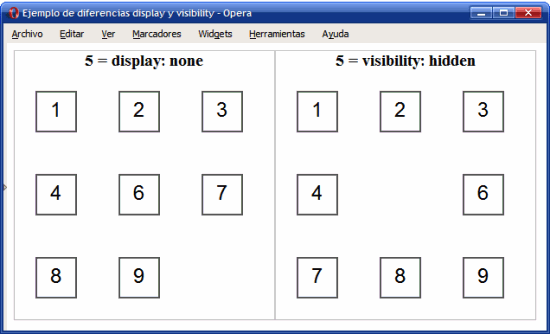
\includegraphics[width=0.8\textwidth]{img/f0522.png}
\end{figure}
\end{center}

\end{frame}


%%---------------------------------------------------------------

\begin{frame}
\frametitle{Propiedad display}

\begin{center}
  \begin{table}
   \begin{tabular}{p{1.8cm}p{7.8cm}}
Propiedad & \bf{display} \\ \hline
Valores& inline | block | none | list-item | run-in | inline-block | table | inline-table | table-row-group | table-header-group | table-footer-group | table-row | table-column-group | table-column | table-cell | table-caption | inherit \\ \hline
Se aplica a& Todos los elementos \\ \hline
Valor inicial& inline \\ \hline
Descripción& Permite controlar la forma de visualizar un elemento e incluso ocultarlo \\ \hline
  \end{tabular}
   \caption{Definición de la propiedad display de CSS}
 \end{table}
\end{center}


\end{frame}




%%---------------------------------------------------------------

\begin{frame}
\frametitle{Propiedad visibility}

\begin{center}
  \begin{table}
   \begin{tabular}{p{1.8cm}p{7.8cm}}
Propiedad & \bf{visibility} \\ \hline
Valores& visible | hidden | collapse | inherit \\ \hline
Se aplica a& Todos los elementos \\ \hline
Valor inicial& visible \\ \hline
Descripción& Permite hacer visibles e invisibles a los elementos \\ \hline
  \end{tabular}
   \caption{Definición de la propiedad visibility de CSS}
 \end{table}
\end{center}


\end{frame}


%%---------------------------------------------------------------

\begin{frame}
\frametitle{Propiedad overflow}

\begin{itemize}
  \item En algunas ocasiones el contenido de un elemento no cabe en el espacio reservado para ese elemento y se desborda.
  \item La situación más habitual en la que el contenido sobresale de su espacio reservado es cuando se establece la anchura y/o altura de un elemento mediante la propiedad width y/o height. 
  \item Los valores de la propiedad overflow tienen el siguiente significado:
  \begin{itemize}
    \item visible: el contenido no se corta y se muestra sobresaliendo la zona reservada para visualizar el elemento. Este es el comportamiento por defecto.
    \item hidden: el contenido sobrante se oculta y sólo se visualiza la parte del contenido que cabe dentro de la zona reservada para el elemento.
    \item scroll: solamente se visualiza el contenido que cabe dentro de la zona reservada para el elemento, pero también se muestran barras de scroll que permiten visualizar el resto del contenido.
    \item auto: el comportamiento depende del navegador, aunque normalmente es el mismo que la propiedad scroll.
  \end{itemize}
\end{itemize}

\end{frame}


%%---------------------------------------------------------------

\begin{frame}
\frametitle{Propiedad overflow (y II)}

\begin{center}
\begin{figure}[p]
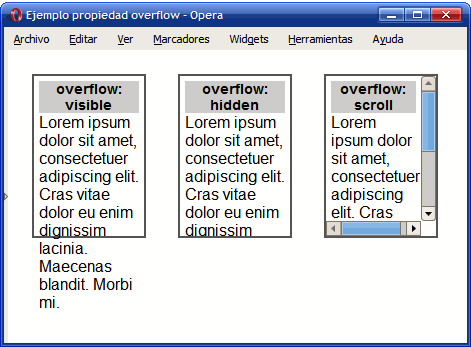
\includegraphics[width=0.8\textwidth]{img/f0524.png}
\end{figure}
\end{center}

\end{frame}


%%---------------------------------------------------------------

\begin{frame}
\frametitle{Propiedad overflow (y III)}

\begin{center}
  \begin{table}
   \begin{tabular}{p{1.8cm}p{7.8cm}}
Propiedad & \bf{overflow} \\ \hline
Valores& visible | hidden | scroll | auto | inherit \\ \hline
Se aplica a& Elementos de bloque y celdas de tablas \\ \hline
Valor inicial& visible \\ \hline
Descripción& Permite controlar los contenidos sobrantes de un elemento \\ \hline
  \end{tabular}
   \caption{Definición de la propiedad overflow de CSS}
 \end{table}
\end{center}


\end{frame}



%%---------------------------------------------------------------

\begin{frame}
\frametitle{Propiedad z-index}

\begin{itemize}
  \item CSS permite controlar la posición tridimensional de las cajas posicionadas
  \item Es posible indicar las cajas que se muestran delante o detrás de otras cajas cuando se producen solapamientos.
  \item Cuanto más alto sea el valor numérico, más cerca del usuario se muestra la caja.
\end{itemize}

\end{frame}


%%---------------------------------------------------------------

\begin{frame}
\frametitle{Propiedad z-index (II)}


\begin{center}
\begin{figure}[p]
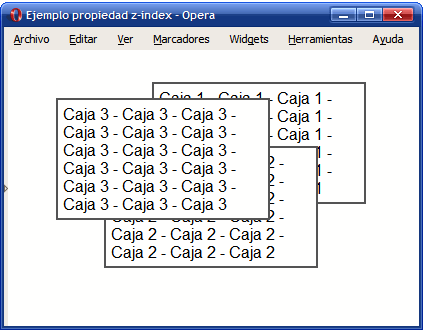
\includegraphics[width=0.66\textwidth]{img/f0525.png}
\end{figure}
\end{center}

\end{frame}



%%---------------------------------------------------------------

\begin{frame}
\frametitle{Propiedad z-index (y III)}

\begin{center}
  \begin{table}
   \begin{tabular}{p{1.8cm}p{7.8cm}}
Propiedad & \bf{z-index} \\ \hline
Valores& auto | $<numero>$ | inherit \\ \hline
Se aplica a& Elementos que han sido posicionados explícitamente \\ \hline
Valor inicial& auto \\ \hline
Descripción& Establece el nivel tridimensional en el que se muestra el elemento \\ \hline
  \end{tabular}
   \caption{Definición de la propiedad z-index de CSS}
 \end{table}
\end{center}


\end{frame}


%%---------------------------------------------------------------
\section{Texto}

\begin{frame}
\frametitle{Tipografía}

\begin{itemize}
  \item CSS define numerosas propiedades para modificar la apariencia del texto
  \item color se utiliza para establecer el color de la letra
  \item Como el valor de la propiedad color se hereda, normalmente se establece la propiedad color en el elemento body para establecer el color de letra de todos los elementos de la página
 \item font-family se utiliza para indicar el tipo de letra con el que se muestra el texto
  \item Suele definirse como una lista de tipos de letra alternativos separados por comas. El último valor de la lista es el nombre de la familia tipográfica genérica que más se parece al tipo de letra que se quiere utilizar.
\end{itemize}

\end{frame}


%%---------------------------------------------------------------

\begin{frame}
\frametitle{Propiedad color}

\begin{center}
  \begin{table}
   \begin{tabular}{p{1.8cm}p{7.8cm}}
Propiedad & \bf{color} \\ \hline
Valores& $<color>$ | inherit \\ \hline
Se aplica a& Todos los elementos \\ \hline
Valor inicial& Depende del navegador \\ \hline
Descripción& Establece el color de letra utilizado para el texto \\ \hline
  \end{tabular}
   \caption{Definición de la propiedad color de CSS}
 \end{table}
\end{center}


\end{frame}


%%---------------------------------------------------------------

\begin{frame}
\frametitle{Propiedad font-family}

\begin{center}
  \begin{table}
   \begin{tabular}{p{1.8cm}p{7.8cm}}
Propiedad & \bf{font-family} \\ \hline
Valores& (( $<nombre\_familia>$ | $<familia\_generica>$ ) (,$nombre\_familia>$ | $<familia\_generica$)* ) | inherit \\ \hline
Se aplica a& Todos los elementos \\ \hline
Valor inicial& Depende del navegador \\ \hline
Descripción& Establece el tipo de letra utilizado para el texto \\ \hline
  \end{tabular}
   \caption{Definición de la propiedad font-family de CSS}
 \end{table}
\end{center}


\end{frame}


%%---------------------------------------------------------------

\begin{frame}
\frametitle{Propiedad font-size (I)}

\begin{itemize}
  \item Además de medida relativas, absolutas y de porcentajes, CSS permite utilizar una serie de palabras clave para indicar el tamaño de letra del texto:
  \begin{itemize}
    \item tamaño\_absoluto: indica el tamaño de letra de forma absoluta mediante alguna de las siguientes palabras clave: xx-small, x-small, small, medium, large, x-large, xx-large.
    \item tamaño\_relativo: indica de forma relativa el tamaño de letra del texto mediante dos palabras clave (larger, smaller) que toman como referencia el tamaño de letra del elemento padre.
  \end{itemize}
\end{itemize}


\begin{center}
\begin{figure}[p]
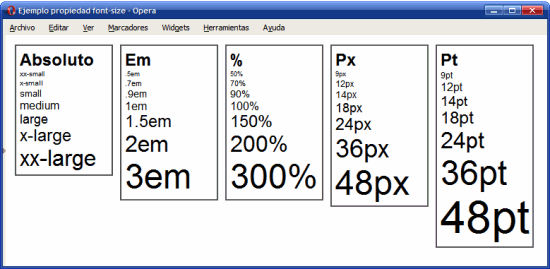
\includegraphics[width=0.6\textwidth]{img/f0601.png}
\end{figure}
\end{center}

\end{frame}


%%---------------------------------------------------------------

\begin{frame}
\frametitle{Propiedad font-size (y II)}

\begin{center}
  \begin{table}
   \begin{tabular}{p{1.8cm}p{7.8cm}}
Propiedad & \bf{font-size} \\ \hline
Valores & $<tamano\_absoluto>$ | $<tamano\_relativo>$ | $<medida>$ | $<porcentaje>$ | inherit \\ \hline
Se aplica a & Todos los elementos \\ \hline
Valor inicial & medium \\ \hline
Descripción & Establece el tamaño de letra utilizado para el texto \\ \hline
  \end{tabular}
   \caption{Definición de la propiedad font-size de CSS}
 \end{table}
\end{center}

\end{frame}


%%---------------------------------------------------------------

\begin{frame}
\frametitle{Propiedad font-weight}

\begin{center}
  \begin{table}
   \begin{tabular}{p{1.8cm}p{7.8cm}}
Propiedad & \bf{font-weight} \\ \hline
Valores& normal | bold | bolder | lighter | 100 | 200 | 300 | 400 | 500 | 600 | 700 | 800 | 900 | inherit \\ \hline
Se aplica a& Todos los elementos \\ \hline
Valor inicial& normal \\ \hline
Descripción& Establece la anchura de la letra utilizada para el texto \\ \hline
  \end{tabular}
   \caption{Definición de la propiedad font-weight de CSS}
 \end{table}
\end{center}


\end{frame}


%%---------------------------------------------------------------

\begin{frame}
\frametitle{Propiedad font-style}

\begin{center}
  \begin{table}
   \begin{tabular}{p{1.8cm}p{7.8cm}}
Propiedad & \bf{font-style} \\ \hline
Valores& normal | italic | oblique | inherit \\ \hline
Se aplica a& Todos los elementos \\ \hline
Valor inicial& normal \\ \hline
Descripción& Establece el estilo de la letra utilizada para el texto \\ \hline
  \end{tabular}
   \caption{Definición de la propiedad font-style de CSS}
 \end{table}
\end{center}

\end{frame}


%%---------------------------------------------------------------

\begin{frame}
\frametitle{Propiedad font-variant}

\begin{center}
  \begin{table}
   \begin{tabular}{p{1.8cm}p{7.8cm}}
Propiedad & \bf{font-variant} \\ \hline
Valores& normal | small-caps | inherit \\ \hline
Se aplica a& Todos los elementos \\ \hline
Valor inicial& normal \\ \hline
Descripción& Establece el estilo alternativo de la letra utilizada para el texto \\ \hline
  \end{tabular}
   \caption{Definición de la propiedad font-variant de CSS}
 \end{table}
\end{center}


\end{frame}


%%---------------------------------------------------------------

\begin{frame}
\frametitle{Propiedad "short-hand" font}

\begin{center}
  \begin{table}
   \begin{tabular}{p{1.8cm}p{7.8cm}}
Propiedad & \bf{font} \\ \hline
Valores& ( ( $<font-style>$ || $<font-variant>$ || $<font-weight>$ )? $<font-size>$ ( / $<line-height>$ )? $<font-family>$ ) | caption | icon | menu | message-box | small-caption | status-bar | inherit \\ \hline
Se aplica a& Todos los elementos \\ \hline
Valor inicial& - \\ \hline
Descripción& Permite indicar de forma directa todas las propiedades de la tipografía de un texto \\ \hline
  \end{tabular}
   \caption{Definición de la propiedad font de CSS}
 \end{table}
\end{center}


\end{frame}


%%---------------------------------------------------------------

\begin{frame}[fragile]
\frametitle{Propiedad "short-hand" font (y II)}

\begin{itemize}
  \item El orden en el que se deben indicar las propiedades del texto es el siguiente:
  \begin{itemize}
    \item En primer lugar y de forma opcional se indican el font-style, font-variant y font-weight en cualquier orden.
    \item A continuación, se indica obligatoriamente el valor de font-size seguido opcionalmente por el valor de line-height.
    \item Por último, se indica obligatoriamente el tipo de letra a utilizar.
  \end{itemize}
\end{itemize}

\begin{footnotesize}
\begin{verbatim}
font: bold 1em "Trebuchet MS",Arial,Sans-Serif;
font: normal 0.9em "Lucida Grande", Verdana, Arial, Helvetica, sans-serif;
font: normal 1.2em/1em helvetica, arial, sans-serif;
\end{verbatim}
\end{footnotesize}

\end{frame}


%%---------------------------------------------------------------

\begin{frame}
\frametitle{Texto}

\begin{itemize}
  \item Además de las propiedades relativas a la tipografía del texto, CSS define numerosas propiedades que determinan la apariencia del texto en su conjunto. Estas propiedades adicionales permiten controlar al alineación del texto, el interlineado, la separación entre palabras, etc.
\end{itemize}

\end{frame}


%%---------------------------------------------------------------

\begin{frame}
\frametitle{Propiedad text-align}

\begin{center}
  \begin{table}
   \begin{tabular}{p{1.8cm}p{7.8cm}}
Propiedad & \bf{text-align} \\ \hline
Valores& left | right | center | justify | inherit \\ \hline
Se aplica a& Elementos de bloque y celdas de tabla \\ \hline
Valor inicial& left \\ \hline
Descripción& Establece la alineación del contenido del elemento \\ \hline
  \end{tabular}
   \caption{Definición de la propiedad text-align de CSS}
 \end{table}
\end{center}


\end{frame}


%%---------------------------------------------------------------

\begin{frame}
\frametitle{Propiedad line-height}

\begin{center}
  \begin{table}
   \begin{tabular}{p{1.8cm}p{7.8cm}}
Propiedad & \bf{line-height} \\ \hline
Valores& normal | $<numero>$ | $<medida>$ | $<porcentaje>$ | inherit \\ \hline
Se aplica a& Todos los elementos \\ \hline
Valor inicial& normal \\ \hline
Descripción& Permite establecer la altura de línea de los elementos \\ \hline
  \end{tabular}
   \caption{Definición de la propiedad line-height de CSS}
 \end{table}
\end{center}


\end{frame}


%%---------------------------------------------------------------

\begin{frame}
\frametitle{Propiedad text-decoration}

\begin{center}
  \begin{table}
   \begin{tabular}{p{1.8cm}p{7.8cm}}
Propiedad & \bf{text-decoration} \\ \hline
Valores& none | ( underline || overline || line-through || blink ) | inherit \\ \hline
Se aplica a& Todos los elementos \\ \hline
Valor inicial& none \\ \hline
Descripción& Establece la decoración del texto (subrayado, tachado, parpadeante, etc.) \\ \hline
  \end{tabular}
   \caption{Definición de la propiedad text-decoration de CSS}
 \end{table}
\end{center}


\end{frame}


%%---------------------------------------------------------------

\begin{frame}
\frametitle{Propiedad text-transform}

\begin{center}
  \begin{table}
   \begin{tabular}{p{1.8cm}p{7.8cm}}
Propiedad & \bf{text-transform} \\ \hline
Valores& capitalize | uppercase | lowercase | none | inherit \\ \hline
Se aplica a& Todos los elementos \\ \hline
Valor inicial& none \\ \hline
Descripción& Transforma el texto original (lo transforma a mayúsculas, a minúsculas, etc.) \\ \hline
  \end{tabular}
   \caption{Definición de la propiedad text-transform de CSS}
 \end{table}
\end{center}


\end{frame}


%%---------------------------------------------------------------

\begin{frame}
\frametitle{Propiedad vertical-align}

\begin{center}
  \begin{table}
   \begin{tabular}{p{1.8cm}p{7.8cm}}
Propiedad & \bf{vertical-align} \\ \hline
Valores& baseline | sub | super | top | text-top | middle | bottom | text-bottom | $<porcentaje>$ | $<medida>$ | inherit \\ \hline
Se aplica a& Elementos en línea y celdas de tabla \\ \hline
Valor inicial& baseline \\ \hline
Descripción& Determina la alineación vertical de los contenidos de un elemento \\ \hline
  \end{tabular}
   \caption{Definición de la propiedad vertical-align de CSS}
 \end{table}
\end{center}


\end{frame}


%%---------------------------------------------------------------

\begin{frame}
\frametitle{Propiedad text-indent}

\begin{center}
  \begin{table}
   \begin{tabular}{p{1.8cm}p{7.8cm}}
Propiedad & \bf{text-indent} \\ \hline
Valores& $<medida>$ | $<porcentaje>$ | inherit \\ \hline
Se aplica a& Los elementos de bloque y las celdas de tabla \\ \hline
Valor inicial& 0 \\ \hline
Descripción& Tabula desde la izquierda la primera línea del texto original \\ \hline
  \end{tabular}
   \caption{Definición de la propiedad text-indent de CSS}
 \end{table}
\end{center}


\end{frame}


%%---------------------------------------------------------------

\begin{frame}
\frametitle{Propiedad letter-spacing}

\begin{center}
  \begin{table}
   \begin{tabular}{p{1.8cm}p{7.8cm}}
Propiedad & \bf{letter-spacing} \\ \hline
Valores& normal | $<medida>$ | inherit \\ \hline
Se aplica a& Todos los elementos \\ \hline
Valor inicial& normal \\ \hline
Descripción& Permite establecer el espacio entre las letras que forman las palabras del texto \\ \hline
  \end{tabular}
   \caption{Definición de la propiedad letter-spacing de CSS}
 \end{table}
\end{center}


\end{frame}


%%---------------------------------------------------------------

\begin{frame}
\frametitle{Propiedad word-spacing}

\begin{center}
  \begin{table}
   \begin{tabular}{p{1.8cm}p{7.8cm}}
Propiedad & \bf{word-spacing} \\ \hline
Valores& normal | $<medida>$ | inherit \\ \hline
Se aplica a& Todos los elementos \\ \hline
Valor inicial& normal \\ \hline
Descripción& Permite establecer el espacio entre las palabras que forman el texto \\ \hline
  \end{tabular}
   \caption{Definición de la propiedad word-spacing de CSS}
 \end{table}
\end{center}


\end{frame}


%%---------------------------------------------------------------

\begin{frame}
\frametitle{Propiedad white-space}

\begin{center}
  \begin{table}
   \begin{tabular}{p{1.8cm}p{7.8cm}}
Propiedad & \bf{white-space} \\ \hline
Valores& normal | pre | nowrap | pre-wrap | pre-line | inherit \\ \hline
Se aplica a& Todos los elementos \\ \hline
Valor inicial& normal \\ \hline
Descripción& Establece el tratamiento de los espacios en blanco del texto \\ \hline
  \end{tabular}
   \caption{Definición de la propiedad white-space de CSS}
 \end{table}
\end{center}


\end{frame}


%%---------------------------------------------------------------

\begin{frame}
\frametitle{Propiedad white-space (y II)}

El significado de cada uno de los valores es el siguiente:
\begin{itemize}
  \item normal: comportamiento por defecto de HTML.
  \item pre: se respetan los espacios en blanco y las nuevas líneas (exactamente igual que la etiqueta <pre>). Si la línea es muy larga, se sale del espacio asignado para ese contenido.
  \item nowrap: elimina los espacios en blanco y las nuevas líneas. Si la línea es muy larga, se sale del espacio asignado para ese contenido.
  \item pre-wrap: se respetan los espacios en blanco y las nuevas líneas, pero ajustando cada línea al espacio asignado para ese contenido.
  \item pre-line: elimina los espacios en blanco y respeta las nuevas líneas, pero ajustando cada línea al espacio asignado para ese contenido.
\end{itemize}

\end{frame}


%%---------------------------------------------------------------
\section{Enlaces}

\begin{frame}
\frametitle{Pseudo-clases en enlaces}

Como con los atributos id o class no es posible aplicar diferentes estilos a un mismo elemento en función de su estado, CSS introduce un nuevo concepto llamado pseudo-clases. En concreto, CSS define las siguientes cuatro pseudo-clases:

\begin{itemize}
  \item :link, aplica estilos a los enlaces que apuntan a páginas o recursos que aún no han sido visitados por el usuario.
  \item :visited, aplica estilos a los enlaces que apuntan a recursos que han sido visitados anteriormente por el usuario. El historial de enlaces visitados se borra automáticamente cada cierto tiempo y el usuario también puede borrarlo manualmente.
  \item :hover, aplica estilos al enlace sobre el que el usuario ha posicionado el puntero del ratón.
  \item :active, aplica estilos al enlace que está pinchando el usuario. Los estilos sólo se aplican desde que el usuario pincha el botón del ratón hasta que lo suelta.
\end{itemize}

\end{frame}


%%---------------------------------------------------------------

\begin{frame}
\frametitle{Imágenes según el estilo del enlace}

\begin{itemize}
  \item En ocasiones, puede resultar útil incluir un pequeño icono al lado de un enlace para indicar el tipo de contenido que enlaza.
  \item Este tipo de imágenes son puramente decorativas en vez de imágenes de contenido, por lo que se deberían añadir con CSS y no con elementos de tipo $<img>$. Utilizando la propiedad background (y background-image) se puede personalizar el aspecto de los enlaces para que incluyan un pequeño icono a su lado.
  \item La técnica consiste en mostrar una imagen de fondo sin repetición en el enlace y añadir el padding necesario al texto del enlace para que no se solape con la imagen de fondo.
\end{itemize}

\end{frame}


%%---------------------------------------------------------------

\begin{frame}[fragile]
\frametitle{Imágenes según el estilo del enlace (II)}

\begin{footnotesize}
\begin{verbatim}
a { margin: 1em 0; float: left; clear: left; }
 
.rss {
  color: #E37529;
  padding: 0 0 0 18px;
  background: #FFF url(imagenes/rss.gif) no-repeat left center;
}
 
.pdf {
  padding: 0 0 0 22px;
  background: #FFF url(imagenes/pdf.png) no-repeat left center;
}
 
<a href="#">Enlace con el estilo por defecto</a>
<a class="rss" href="#">Enlace a un archivo RSS</a>
<a class="pdf" href="#">Enlace a un documento PDF</a>
\end{verbatim}
\end{footnotesize}

\end{frame}

%%---------------------------------------------------------------

\begin{frame}
\frametitle{Imágenes según el estilo del enlace (y III)}


\begin{center}
\begin{figure}[p]
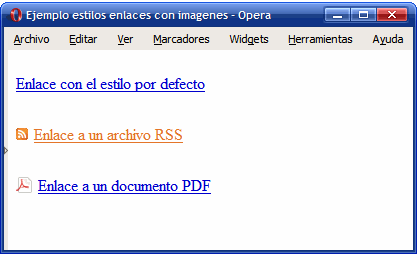
\includegraphics[width=0.8\textwidth]{img/f0704.png}
\end{figure}
\end{center}

\end{frame}


%%---------------------------------------------------------------

\begin{frame}[fragile]
\frametitle{Mostrar los enlaces como si fueran botones}

\begin{footnotesize}
\begin{verbatim}
a { margin: 1em 0; float: left; clear: left; }
a.boton {
  text-decoration: none;
  background: #EEE;
  color: #222;
  border: 1px outset #CCC;
  padding: .1em .5em;
}
a.boton:hover {
  background: #CCB;
}
a.boton:active {
  border: 1px inset #000;
}
<a class="boton" href="#">Guardar</a>
<a class="boton" href="#">Enviar</a>
\end{verbatim}
\end{footnotesize}

\end{frame}


%%---------------------------------------------------------------

\section{Listas}

\begin{frame}
\frametitle{Propiedad list-style-type}

\begin{center}
  \begin{table}
   \begin{tabular}{p{1.8cm}p{7.8cm}}
Propiedad & \bf{list-style-type} \\ \hline
Valores& disc | circle | square | decimal | decimal-leading-zero | lower-roman | upper-roman | lower-greek | lower-latin | upper-latin | armenian | georgian | lower-alpha | upper-alpha | none | inherit \\ \hline
Se aplica a& Elementos de una lista \\ \hline
Valor inicial& disc \\ \hline
Descripción& Permite establecer el tipo de viñeta mostrada para una lista \\ \hline
  \end{tabular}
   \caption{Definición de la propiedad list-style-type de CSS}
 \end{table}
\end{center}


\end{frame}


%%---------------------------------------------------------------

\begin{frame}
\frametitle{Propiedad list-style-position}

\begin{center}
  \begin{table}
   \begin{tabular}{p{1.8cm}p{7.8cm}}
Propiedad & \bf{list-style-position} \\ \hline
Valores& inside | outside | inherit \\ \hline
Se aplica a& Elementos de una lista \\ \hline
Valor inicial& outside \\ \hline
Descripción& Permite establecer la posición de la viñeta de cada elemento de una lista \\ \hline
  \end{tabular}
   \caption{Definición de la propiedad list-style-type de CSS}
 \end{table}
\end{center}


\end{frame}


%%---------------------------------------------------------------

\begin{frame}
\frametitle{Propiedad list-style-image}

\begin{center}
  \begin{table}
   \begin{tabular}{p{1.8cm}p{7.8cm}}
Propiedad & \bf{list-style-image} \\ \hline
Valores& $<url>$ | none | inherit \\ \hline
Se aplica a& Elementos de una lista \\ \hline
Valor inicial& none \\ \hline
Descripción& Permite reemplazar las viñetas automáticas por una imagen personalizada \\ \hline
  \end{tabular}
   \caption{Definición de la propiedad list-style-image de CSS}
 \end{table}
\end{center}


\end{frame}


%%---------------------------------------------------------------

\begin{frame}
\frametitle{Propiedad "shorthand" list-style}

\begin{center}
  \begin{table}
   \begin{tabular}{p{1.8cm}p{7.8cm}}
Propiedad & \bf{list-style} \\ \hline
Valores& ( $<list-style-type>$ || $<list-style-position>$ || $<list-style-image>$ ) | inherit \\ \hline
Se aplica a& Elementos de una lista \\ \hline
Valor inicial& - \\ \hline
Descripción& Propiedad que permite establecer de forma simultánea todas las opciones de una lista \\ \hline
  \end{tabular}
   \caption{Definición de la propiedad list-style de CSS}
 \end{table}
\end{center}


\end{frame}


%%---------------------------------------------------------------

\begin{frame}
\frametitle{Crear un menú vertical}

\begin{enumerate}
  \item Definir anchura del menú
  \item Eliminar las viñetas automáticas y todos los márgenes y espaciados aplicados por defecto
  \item Añadir un borde al menú de navegación y establecer el color de fondo y los bordes de cada elemento del menú
  \item Aplicar estilos a los enlaces: mostrarlos como un elemento de bloque para que ocupen todo el espacio de cada <li> del menú, añadir un espacio de relleno y modificar los colores y la decoración por defecto
\end{enumerate}


\begin{center}
\begin{figure}[p]
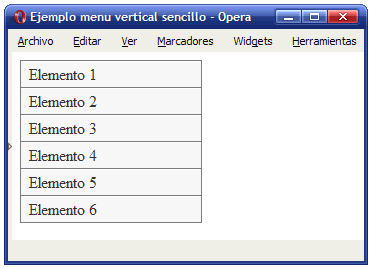
\includegraphics[width=0.6\textwidth]{img/f0908.png}
\end{figure}
\end{center}

\end{frame}


%%---------------------------------------------------------------

\begin{frame}
\frametitle{Menú horizontal básico}

\begin{enumerate}
  \item Aplicar los estilos CSS básicos para establecer el estilo del menú (similares a los del menú vertical)
  \item  Establecer la anchura de los elementos del menú. Si el menú es de anchura variable y contiene cinco elementos, se asigna una anchura del 20\% a cada elemento
  \item Establecer los bordes de los elementos que forman el menú
  \item Se elimina el borde derecho del último elemento de la lista, para evitar el borde duplicado
\end{enumerate}


\begin{center}
\begin{figure}[p]
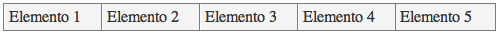
\includegraphics[width=0.8\textwidth]{img/f0909.png}
\end{figure}
\end{center}

\end{frame}


%%---------------------------------------------------------------

%\begin{frame}
%\frametitle{}

%\begin{itemize}
%  \item 
%\end{itemize}
%
%\end{frame}


